\chapter{A numerical tour}\label{ch:numerical_tour}

The goal of this chapter is to display how the theoretical discussion presented thus far relates to the practice of signal recovery on graphs. First of all, I show how to implement the \acrfull{gtv} decoders as efficient iterative procedures derived from a proximal splitting technique. They are efficient in the sense that they require only a sequence of sparse matrix-vector multiplications and some inexpensive elementwise operations. Then, I present four datasets with signals that exhibit small jump-sets with respect to their graph support~\footnote{Recall that small jump-sets are what qualify a graph signal as piecewise-constant.}. The first contains draws of random graphs under the \acrfull{sbm}; the corresponding signals are the community-indicator vectors. The \acrshort{sbm} is traditionally used to emulate clustered networks, so this data could be seen as a sort of baseline for comparisons. The next two datasets have each a single, fixed graph. The \texttt{email-EU-core} network encodes email exchanges across departments in a European research institution; the \texttt{swiss-national-council} network~\footnote{The same from Chapter~\ref{ch:intro}.} connects members of the Swiss Parliament by ``voting similarity''. The piecewise-constant signals in each of these two are derived from the ``natural'' communities in their respective graphs. The final dataset, \texttt{BSDS300}, relates to an image segmentation task. Each graph in this collection represents a natural image by mapping pixels to vertices and patch color similarity to edges. The images' segmentation masks can then be interpreted as piecewise-constant graph signals. The second half of the chapter is a series of numerical experiments on our four datasets. For information on how to reproduce them, visit
\begin{center}
    \framebox[1.1\width][c]{%
        \parbox[t][22pt][c]{0.9\textwidth}{\url{https://github.com/rodrigo-pena/phd-thesis/blob/master/python/README.md}}
}
\end{center}
To supplement a discussion from Chapter \ref{ch:recovery_convex}, I show how the behavior of the interpolation error changes if we minimize the \acrshort{gtv} semi-norm $\|\mathbf{D} \cdot\|_1$ or the Dirichlet form $\|\mathbf{D} \cdot\|_2^2$. Under \acrshort{gtv} minimization, the recovery error goes through a sharp phase transition as the number of measurements increases; under the Dirichlet form, the error decays smoothly. The main set of experiments then investigates the sampling design's effect over the recovery error of \acrshort{gtv} interpolation. For that I compare uniform random sampling with two designs inspired by the results of Chapter~\ref{ch:inexact_dual}. To reduce the number of samples needed for recovery, the experiments show that it is important to know more about the signal's jump-set than just its size.


\section{Implementing the \texorpdfstring{\acrshort{gtv}}{G-TV} decoders with proximal splitting}

There is a base algorithm that can be used to solve both~\footnote{Here I incur in a slight abuse of notation, which was already foreseen in Chapter~\ref{ch:graphs_signals_sampling}, Section~\ref{sec:sampling}. Still (from the implementation's perspective) it is more convenient to work with the square projection operator $\mathbf{P}_{\Omega} \in \mathbb{R}^{n \times n}$ than with the rectangular sampling matrix $\mathbf{A} \in \mathbb{R}^{m \times n}$. Through zero-padding, one can avoid ever going from $\mathbb{R}^{n}$ to $\mathbb{R}^{m}$. Furthermore, identifying $\mathbf{A}$ with $\mathbf{P}_{\Omega}$ turns matrices like $\mathbf{A}^\top \mathbf{A}$ --- that would appear in the algorithms --- into $\mathbf{P}_{\Omega}^\top \mathbf{P}_{\Omega} = \mathbf{P}_{\Omega}$, because the later is a projection operator. Overall, the algorithms' statement is cleaner using $\mathbf{P}_{\Omega}$.}
\begin{equation}
    \underset{\mathbf{z} \in \mathbb{R}^{n}}{\min} \| \mathbf{D z} \|_1 \text{ such that } \mathbf{P}_{\Omega}\mathbf{z} = \mathbf{P}_{\Omega}\mathbf{x} \tag{P1}
\end{equation}
and
\begin{equation}
    \underset{\mathbf{z} \in \mathbb{R}^{n}}{\min}  \| \mathbf{D z} \|_1 \text{ subject to } \| \mathbf{P}_{\Omega}\mathbf{z} - \mathbf{y} \|_q^q \leq \eta \tag{P1-$\eta$}.
\end{equation}
To use it, I need to state each of these problems in the generic unconstrained form
\begin{equation}\label{eq:standard_primal_dual}
    \underset{\mathbf{z} \in \mathbb{R}^{n}}{\min} \enspace f(\mathbf{z}) + g(\mathbf{Dz}) + h(\mathbf{z})
\end{equation}
using convex functions $f: \mathbb{R}^{n} \to \mathbb{R}$ and $g: \mathbb{R}^{N} \to \mathbb{R}$, and a function $h: \mathbb{R}^{n} \to \mathbb{R}$ that is both convex \emph{and} differentiable. I will do that first for problem \eqref{eq:l1_interpolation}, with help from a \emph{convex indicator function}.

\begin{definition}[Convex indicator function]
    The convex indicator function of a set $\mathcal{C}$ is the mapping
    \begin{equation}
        \mathbf{z} \mapsto \iota_{\mathcal{C}}(\mathbf{z}) = \left \{
            \begin{matrix}
                0, & \text{if} \enspace \mathbf{z} \in \mathcal{C}, \\
                +\infty & \text{otherwise}.
            \end{matrix}
        \right.
    \end{equation}
\end{definition}

This function is useful whenever one needs to transform a constrained problem like $\underset{\mathbf{z} \in \mathcal{C}}{\min} \enspace f(\mathbf{z})$ into its unconstrained equivalent $\underset{\mathbf{z} \in \mathbb{R}^{n}}{\min} \enspace f(\mathbf{z}) + \iota_{\mathcal{C}}(\mathbf{z})$. The \emph{interpolation} problem has a constraint set $\mathcal{C} := \{ \mathbf{z} \in \mathbb{R}^{n} : \mathbf{P}_{\Omega}\mathbf{z} = \mathbf{P}_{\Omega} \mathbf{x}\}$, so the template \eqref{eq:standard_primal_dual} represents \eqref{eq:l1_interpolation} if we set
\begin{align}
    f(\cdot) & = \iota_{\{ \mathbf{z} \in \mathbb{R}^{n} : \mathbf{P}_{\Omega}\mathbf{z} = \mathbf{P}_{\Omega} \mathbf{x}\}}(\cdot) \\
    g(\cdot) & = \| \cdot \|_1 \\
    h(\cdot) & \equiv 0.
\end{align}

For the \emph{regression} problem, I will proceed differently. Let us focus on the case when $q = 2$ in the error estimate, so that $\mathbf{z} \mapsto \left\|\mathbf{P}_{\Omega} \mathbf{z} - \mathbf{y}\right\|_2^2$ is a convex, differentiable function. Then there is some regularization hyperparameter $\rho$ for which the choice
\begin{align}
    f(\cdot) & = 0 \\
    g(\cdot) & = \| \cdot \|_1 \\
    h(\cdot) & = \frac{\rho}{2} \| \mathbf{P}_{\Omega} (\cdot) - \mathbf{y}\|_2^2
\end{align}
expresses in \eqref{eq:standard_primal_dual} the same problem as \eqref{eq:l1_regression}~\cite[Ch. 5]{boyd2009}.

The \acrfull{fbf} primal-dual procedure in Komodakis~and~Pesquet~\cite[Algorithm~6]{komodakis2015} is a numerical solver for any problem of the form \eqref{eq:standard_primal_dual}. It is based on a proximal splitting technique, alternating between (forward) gradient steps and (backward) calls to a proximity operator. Between each forward and backward steps the matrix $\mathbf{D}$ connects the primal and dual spaces.~\footnote{The primal space in our problems is $\mathbb{R}^{n}$ (where $\mathbf{x}$ lives), while the dual space is $\mathbb{R}^{N}$ (the co-domain of $\mathbf{D}$).} Interested readers can find a more detailed account in Appendix \ref{ap:primal_dual_prox_split}. Meanwhile, I present Algorithms \ref{algo:primal_dual_interpolation} and \ref{algo:primal_dual_regression} as the respective translations of the base \acrshort{fbf} procedure for the particular problems \eqref{eq:l1_interpolation} and \eqref{eq:l1_regression}. Therein, $\operatorname{soft}_{\gamma} (\cdot)$ represents the soft thresholding operation, defined coordinatewise by
\begin{equation*}
    \forall i, \enspace w_i \mapsto \left\{
        \begin{matrix}
            w_i - \gamma, & \text{if } w_i > \gamma\\
            0, & \text{if } |w_i| \leq \gamma\\
            w_i + \gamma, & \text{if } w_i < -\gamma
        \end{matrix}
    \right. .
\end{equation*}
This function shows up because it is the proximity operator associated with the $\ell_1$ norm. The algorithms admit some leeway in specifying the step sizes for each iteration. As long as the sequence $(\gamma_n)_{n \in \mathbb{N}}$ stays within the given intervals, convergence is guaranteed~\cite{komodakis2015}.

\begin{algorithm}[H]
    \caption{\acrshort{fbf} primal-dual iterations for solving \eqref{eq:l1_interpolation}}
    \label{algo:primal_dual_interpolation}
    \begin{algorithmic}[1]
        \State{$\mathbf{z}_0 \gets \mathbf{0} \in \mathbb{R}^{n}$}\Comment{Primal variable}
        \State{$\mathbf{d}_0 \gets \mathbf{0} \in \mathbb{R}^{N}$}\Comment{Dual variable}
        \Repeat
            \State{\textbf{pick} $\gamma_n \in \left(0, \frac{1}{1 + \|\mathbf{D}\|_{2}}\right)$}

            \State{$\left(\mathbf{w}_{1,n},\enspace\mathbf{w}_{2,n}\right) \gets \left(\mathbf{z}_n - \gamma_n \mathbf{D}^\top \mathbf{d}_n,\enspace\mathbf{d}_n + \gamma_n \mathbf{D}\mathbf{z}_n\right)$}\Comment{Forward}

            \State{$\left(\mathbf{p}_{{1,n}},\enspace\mathbf{p}_{{2,n}}\right) \gets \left((\mathbf{I}_n - \mathbf{P}_{\Omega}) \mathbf{w}_{1,n} + \mathbf{P}_{\Omega} \mathbf{x},\enspace\mathbf{w}_{2,n} - \operatorname{soft}_{\gamma_n} (\mathbf{w}_{2,n})\right)$}\Comment{Backward}

            \State{$\left(\mathbf{q}_{{1,n}},\enspace\mathbf{q}_{{2,n}}\right) \gets \left(\mathbf{p}_{{1,n}} - \gamma_n \mathbf{D}^\top \mathbf{p}_{{2,n}},\enspace\mathbf{p}_{{2,n}} + \gamma_n \mathbf{D} \mathbf{p}_{{1,n}}\right)$}\Comment{Forward}

            \State{$\left(\mathbf{z}_{n+1},\enspace\mathbf{d}_{n+1}\right) \gets \left(\mathbf{z}_n - \mathbf{w}_{1,n} + \mathbf{q}_{1,n},\enspace\mathbf{d}_n - \mathbf{w}_{2,n} + \mathbf{q}_{2,n}\right)$}

        \Until{convergence}
        \State{\textbf{return} $\mathbf{z}_{n+1}$}
	\end{algorithmic}
\end{algorithm}

\begin{algorithm}[H]
    \caption{\acrshort{fbf} primal-dual iterations for solving \eqref{eq:l1_regression}}
    \label{algo:primal_dual_regression}
    \begin{algorithmic}[1]
        \State{$\mathbf{z}_0 \gets \mathbf{0} \in \mathbb{R}^{n}$}\Comment{Primal variable}
        \State{$\mathbf{d}_0 \gets \mathbf{0} \in \mathbb{R}^{N}$}\Comment{Dual variable}
        \Repeat
            \State{\textbf{pick} $\gamma_n \in \left(0, \frac{1}{1 + \rho + \|\mathbf{D}\|_{2}}\right)$}

            \State{$\left(\mathbf{w}_{1,n},\enspace\mathbf{w}_{2,n}\right) \gets \left(\mathbf{z}_n - \gamma_n \left[\rho (\mathbf{P}_{\Omega} \mathbf{z}_n - \mathbf{y}) + \mathbf{D}^\top \mathbf{d}_n\right],\enspace\mathbf{d}_n + \gamma_n \mathbf{D}\mathbf{z}_n\right)$}\Comment{Forward}

            \State{$\left(\mathbf{p}_{{1,n}},\enspace\mathbf{p}_{{2,n}}\right) \gets \left(\mathbf{0},\enspace\mathbf{w}_{2,n} - \operatorname{soft}_{\gamma_n} (\mathbf{w}_{2,n})\right)$}\Comment{Backward}

            \State{$\left(\mathbf{q}_{{1,n}},\enspace\mathbf{q}_{{2,n}}\right) \gets \left(\mathbf{p}_{{1,n}} - \gamma_n \left[\rho (\mathbf{P}_{\Omega} \mathbf{z}_n - \mathbf{y}) + \mathbf{D}^\top \mathbf{p}_{{2,n}}\right],\enspace\mathbf{p}_{{2,n}} + \gamma_n \mathbf{D} \mathbf{p}_{{1,n}}\right)$}\Comment{Forward}

            \State{$\left(\mathbf{z}_{n+1},\enspace\mathbf{d}_{n+1}\right) \gets \left(\mathbf{z}_n - \mathbf{w}_{1,n} + \mathbf{q}_{1,n},\enspace\mathbf{d}_n - \mathbf{w}_{2,n} + \mathbf{q}_{2,n}\right)$}

        \Until{convergence}
        \State{\textbf{return} $\mathbf{z}_{n+1}$}
	\end{algorithmic}
\end{algorithm}

Other algorithms could certainly be used to implement \eqref{eq:l1_interpolation} and \eqref{eq:l1_regression}, but the \acrshort{fbf} procedure is good enough for two reasons. The first, I have already mentioned: the same general algorithm applies to both problems. The second reason has to do with numerical efficiency. Each step in Algorithms \ref{algo:primal_dual_interpolation} and \ref{algo:primal_dual_regression} requires only elementwise operations, and matrix-vector multiplications using the graph gradient operator $\mathbf{D}$. Graphs used in practice are often sparse~\footnote{Sparse graphs are ones that have few edges. Generally, graphs are considered sparse their number of edges is on the order of their number of vertices. Dense graphs can have a number of edges on the order of the square of the number of vertices. As the number of vertices grows, storing dense graphs quickly becomes a problem on most systems.}, so that $\mathbf{D}$ has few non-zero entries, making multiplications with it cheap to compute.


\section{The data}

To test the \acrshort{gtv} decoders, we should let them try to recover the sort of signal that motivated their study. Signals with a small jump-set can always be found in the indicator vectors of the communities in a clusterable graph. I present here four datasets, drawn from different domains, yielding graphs with different cluster structure. The clusters are reflected --- in varying degrees --- on the constant pieces of the assembled signals therein. Each dataset in this section is used in at least some experiment later on in the chapter.

\subsection{Community indicator vectors in the \texorpdfstring{\acrlong{sbm}}{Stochastic Block Model}}

The standard way to simulate graphs with a community structure is via the \acrfull{sbm}\footnote{According to Abbe \cite{abbe2018}, this is the most commonly used name for it in the Statistics literature. The model is also known as ``planted partitions'' in Computer Science, or ``inhomogeneous random graph'' in Mathematics.}. The \acrshort{sbm} describes a \emph{distribution} of random graphs, and one may refer to it using the notation \acrshort{sbm}$(n, \mathcal{C}, \mathbf{p}, \mathbf{Q})$ when the drawn graphs have a fixed number $n$ of vertices~\cite{abbe2018}. The set $\mathcal{C} = \{\mathcal{C}_1 , \dots, \mathcal{C}_k \}$ lists the communities, which are themselves lists of vertices in the graph. The vector $\mathbf{p} = (p_1, \dots, p_k)$ lists the probabilities with which vertices within each community connect to each other.~\footnote{For example, let $v_i, v_j$ be two vertices in the same community, $\mathcal{C}_1$, and write $v_i \sim v_j$ if these vertices are connected. Then $\mathbb{P} ( \{  v_i \sim v_j \}) = p_1$.} The matrix $\mathbf{Q}$, in turn, gathers the probabilities of connection across communities.~\footnote{Take $v_i \in \mathcal{C}_1$ again, but $v_j$ in another community, $\mathcal{C}_2$. Then $\mathbb{P} ( \{  v_i \sim v_j \}) = Q_{12}$.}.

In my experiments, I only consider \acrshort{sbm} graphs with two communities, having the same internal connection probability $p$. In other words, $p_1 = p_2 = p$. Since there are only two communities, matrix $\mathbf{Q}$ can be reduced to a single probability parameter $q$. I will use a shorthand and refer to this restricted distribution as \acrshort{sbm}$(n, 2, p, q)$. If the two communities in the model are the same size, they become statistically indistinguishable, or ``symmetric''. I will sometimes highlight this setting by referring to it as 2-\texttt{SSBM}, while calling the (potentially) unbalanced alternative 2-\texttt{SBM}. Note that I might also write the partition of vertices between communities in evidence as a sum of two terms. For example, the unbalanced 2-\texttt{SBM} of Figure~\ref{fig:2ssbm_and_2sbm} has 200 vertices in the first community and 800 in the second, hence the appended ``(200~+~800)''. Balanced or unbalanced, the \acrshort{sbm} experiments always use the indicator vector of the smallest community as the piecewise-constant signal. For matters of graph signal processing, I enforce a unitary edge weight between connected vertices in the \acrshort{sbm} graphs. Thus, their gradient matrix, $\mathbf{D}$, only has entries valued $-1$, $0$, or $1$.

\begin{figure}[H]
    \centering
    \subfloat[Balanced 2-\texttt{SSBM}(500~+~500)]{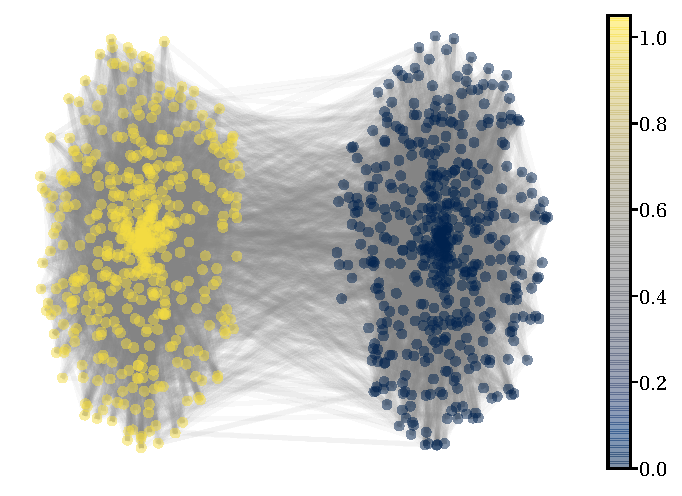
\includegraphics[width=0.48\textwidth]{2ssbm.pdf}}
    \hfill
    \subfloat[Unbalanced 2-\texttt{SBM}(200~+~800)]{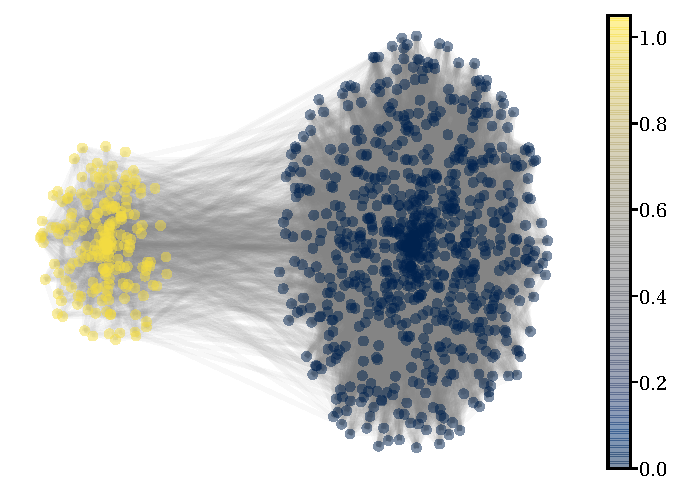
\includegraphics[width=0.48\textwidth]{2sbm.pdf}}
    \caption[Graphs from 2-\texttt{SSBM}(500~+~500) and 2-\texttt{SBM}(200~+~800)]{Graphs drawn from the \acrshort{sbm}$\left(1000, 2, 4.5 \frac{\log (1000)}{1000}, 0.5 \frac{\log (1000)}{1000}\right)$ model, varying the relative community sizes. The vertex colors represent the indicator vector of the leftmost community.}
    \label{fig:2ssbm_and_2sbm}
\end{figure}

My use of community indicator vectors is inspired by one of the basic questions in the study of \acrlongpl{sbm}: can one retrieve the community partitions by looking at the edge structure of graphs drawn from the distribution? Researchers like Abbe~\etal~\cite{abbe2015, abbe2018} have used the \acrfull{map} estimator as a tool prove when this question can be answered. Theorem \ref{thm:exact_recovery_sbm} shows this solvability threshold for the parameters of the 2-\texttt{SSBM}.

\clearpage

\begin{theorem}[\protect{\cite[Thm. 7.1]{abbe2018}}]
    Exact recovery in the symmetric \acrshort{sbm}$\left(n, 2, a \frac{\log n}{n}, b \frac{\log n}{n}\right)$ is solvable if and only if
    \begin{equation}
        \left(\sqrt{a} - \sqrt{b}\right)^2 > 2.
    \end{equation}
    \label{thm:exact_recovery_sbm}
\end{theorem}

To retrieve the community partitions, the graphs drawn from the \acrshort{sbm} distribution have to be at least \emph{connected}~\footnote{Recall from Chapter~\ref{ch:graphs_signals_sampling} that a graph is connected if one can visit all the vertices by travelling only on the edges of the graph.}. Abbe \cite{abbe2018} points out that $a + b > 2$ is the parameter regime for which the 2-\texttt{SSBM} graphs are connected with high probability. The theorem above implies then that $2(\sqrt{ab} - 1)$ is the extra factor needed to go from connectivity to exact recovery. But Abbe's result concerns retrieving the community partitions when all we can observe is the edge structure of the \acrshort{sbm} graphs. When I sample the community indicator vectors, I effectively call upon an oracle to reveal the true assignment of certain vertices. How does the recovery error of the \acrshort{gtv} interpolation \eqref{eq:l1_interpolation} behaves for \acrshort{sbm} distributions with parameter regimes in the neighborhood of the one from Theorem~\ref{thm:exact_recovery_sbm}?

Figure \ref{fig:pt_2ssbm_unif_samp_tv_interp_with_thresholds} shows an initial answer to that question for the 2-\texttt{SSBM}. There, I use uniform random sampling (with replacement) to query the vertex community assignments. The number of measurements varies from zero to the number of vertices~\footnote{Note however that since the sampling is with replacement a number of measurements equal to the number of vertices does not have to yield zero recovery error because there can be redundant samples.}. On the vertical axis, I vary the intra-community connection parameter $a$, starting from the connectivity regime ($a + b > 2$) --- in the bottom --- and passing by the solvability regime from Theorem~\ref{thm:exact_recovery_sbm} --- in the middle. The higher up on the vertical axis, the more dense each community tends to be in terms of number of edges. The average number of edges connecting vertices between different communities stays the same throughout. I measure the recovery error as a normalized~\footnote{The normalization factor is the inverse of the Euclidean norm of the ground-truth signal.} Euclidean distance between the signal estimated by \eqref{eq:l1_interpolation} and the ``ground-truth'' indicator vector. The plot to the right of the figure is a quantized version of the one to the left, presented so that we can better distinguish the level sets in the recovery error.

\begin{figure}[ht]
    \centering
    \subfloat[Recovery error (normalized Euclidean distance)]{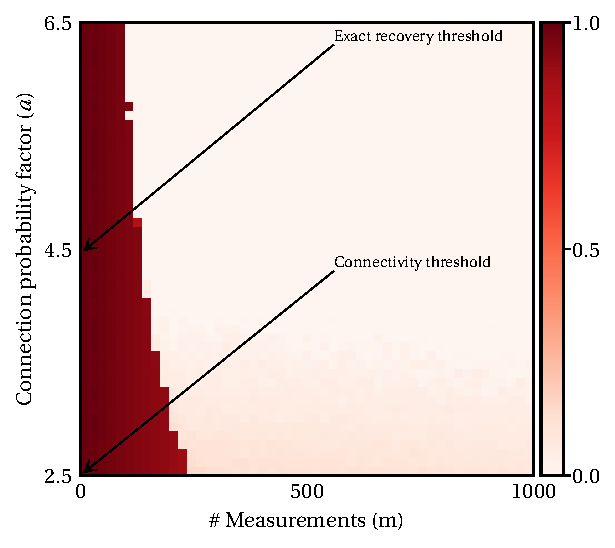
\includegraphics[width=0.48\textwidth]{pt_2ssbm_unif_samp_tv_interp_with_thresholds.pdf}}
    \hfill
    \subfloat[Quantized version]{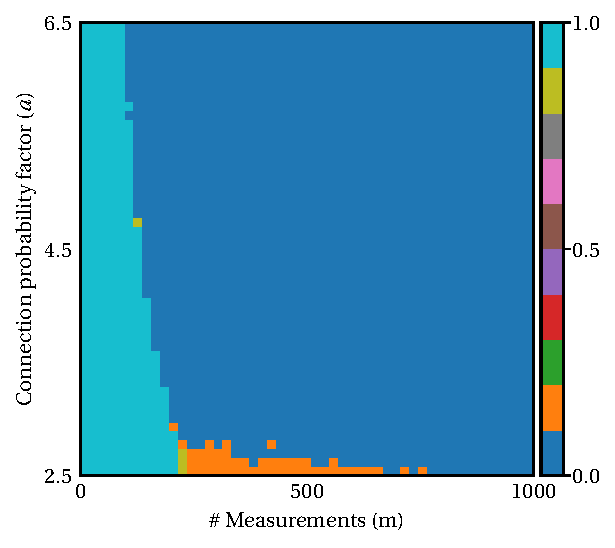
\includegraphics[width=0.48\textwidth]{pt_2ssbm_unif_samp_tv_interp_quantized.pdf}}
    \caption[Phase transition of the recovery error in 2-\texttt{SSBM}(500~+~500) graphs]{Phase transition for the error of \eqref{eq:l1_interpolation} in recovering the community indicator vector of graphs drawn from the symmetric \acrshort{sbm}$\left(1000, 2, a \frac{\log (1000)}{1000}, 0.5 \frac{\log (1000)}{1000}\right)$ from uniform random samples. Each pixel represents the median recovery error across 25 independent trials.}
    \label{fig:pt_2ssbm_unif_samp_tv_interp_with_thresholds}
\end{figure}

Note the clear phase transition when the number of samples reaches a critical value. The threshold happens earlier the higher up on the plot, where the number of edges within the communities becomes progressively larger (on average) than the size of the indicator vector's jump-set. But even the bottom half of the plot exhibits very small recovery errors. This observation does not contradict Theorem \ref{thm:exact_recovery_sbm} --- of course --- but simply attests to the extra information included in the measurements themselves. To allow comparisons with this initial plot, the remaining \acrshort{sbm} experiments in this chapter employ the \acrshort{sbm}$\left(1000, 2, a \frac{\log (1000)}{1000}, 0.5 \frac{\log (1000)}{1000}\right)$ distributions within the same parameter range, \ie with $a$ taking values in the interval $[2.5, 6.5]$.

\subsection{Department indicator vectors in \texttt{email-EU-core}}

The \texttt{email-EU-core} data~\footnote{\url{http://snap.stanford.edu/data/email-Eu-core.html}} represents some email exchanges by people from a large European research institution~\cite{yin2017}. The institution is split into 42 departments, and each of the 1005 individuals in the dataset belongs to exactly one such department. An edge of unitary weight connects two people in the network if they exchanged at least one email. As one could expect, communication tends to stay restricted to within departments, so the network clusters are a reflection the departmental makeup. Thus, the department indicator vectors have small jump sets, as edges across departments are fewer than within. But the number of people in each department is relatively small, so to be fairer with the baseline uniform sampling design I pick as ``ground-truth'' signal for the \texttt{email-EU-core} dataset the indicator vector of the union of the five largest departments. In doing so, the ground-truth takes value $1$ at about 38\% of the vertices and value $0$ at the rest 62\%.

\subsection{Party indicator vectors in \texttt{swiss-national-council}}

I construct the \texttt{swiss-national-council} with data extracted from the 50\textsuperscript{th} legislature in the Swiss Database of Parliamentary Votes~\footnote{\url{https://www.parlament.ch/en/ratsbetrieb/abstimmungen/abstimmungs-datenbank-nr}}. I associate each council member to a feature vector indicating how they voted in each of 3395 affairs accounted for at the time of writing. If they voted \texttt{Yes} in some affair, the corresponding entry in the feature vector receives value $1$; if they voted \texttt{No} the entry gets value $-1$. Affairs for which the councillor did not register a vote (whatever the reason) get a value of $0$. The idea underneath this numerical translation is to use the feature vectors to compare the voting patterns of different council members. Investigating which metric is best for this task is beyond the scope of this thesis, so I opt for the traditional Euclidean distance.

The graph construction takes place directly at the level of the weighted adjacency matrix. Let $\mathbf{f}_i$ and $\mathbf{f}_j$ the the feature vectors of councillors $i$ and $j$. These councillors are then connected with edge weight $W_{ij} = \exp \left ( -\| \mathbf{f}_i - \mathbf{f}_j \|_2^2 / \sigma \right )$, where $\sigma$ is set as the mean distance between feature vectors in the dataset.~\footnote{Exponential kernels such as this are commonly used in Machine Learning and Data Science for similarity computations. The exponential always outputs positive similarity values, and the negative exponent ensures that these values decay quickly towards zero as the feature vectors within become more distant.} Then, to enforce a sparse graph, I keep only the 25 largest edge weights for each council member, setting the rest to $0$ (while making sure that the weight matrix remains symmetric). In the end, councillors that voted identically throughout all the affairs get a unitary edge weight, whereas members that voted differently enough are disconnected.

To put a signal on this graph, I went over the Swiss Parliament files listing the party affiliations of all councillors since 1848.~\footnote{https://www.parlament.ch/en/ratsmitglieder} Intuition tell us that members of the same party stand to vote more similarly than people from different parties. So the party indicator vectors should strongly correlate with the cluster structure of the graph I have constructed. I decided to use as ``ground-truth'' for the experiments the indicator vector of the two largest right-wing parties in the 50\textsuperscript{th} legislature, UDC and FDP. By joining these two parties, the ground-truth signal takes value $1$ at around 46\% of the vertices and $0$ at the other 54\%, an almost even split of the National Council that improves the chances of recovery under uniform random sampling. Meanwhile --- because the two joined parties are to the right in political spectrum --- this concocted ground-truth should still have a sparse jump-set, since the members of UDC and FDP have different voting patterns than the mostly centrist and left-wing politicians in the other half of the Council.

\subsection{Image segmentation masks in \texttt{BSDS300}}

The Berkeley Segmentation Dataset and Benchmark~\footnote{\url{https://www2.eecs.berkeley.edu/Research/Projects/CS/vision/bsds/}} contains 300 images, split into train (100)  and test (200) sets. Each of these images is accompanied by human-generated segmentation masks. What I call the \texttt{BSDS300} dataset is a collection of graphs for each of the 300 images, along with vector representations of the segmentation masks --- interpreted as graph signals.

The first step to construct a graph for each image is to identify each pixel in the image with a vertex in the graph.~\footnote{To get graphs of manageable size for the experiments, I actually subsample the original images by a factor of 12 before starting the graph construction. That is, I keep every 12th row and column of the original image, and use the pixels of this lower-resolution version as the vertices of the graph.} Then, I connect --- with unitary edge weights --- pixels that are adjacent \emph{in the image}. This first set of connection encodes ``spatial similarity'': neighboring pixels in the image are neighbors in the graph. The next set of connections encodes color information via ``patch similarity''. To understand it, let $\mathbf{p}_i \in \mathbb{R}^{147}$ be a vectorized, $7 \times 7 \times 3$ patch containing the RGB values in the image neighborhood centered at pixel $i$.~\footnote{If $i$ is a border pixel, use some form of padding to obtain the patch.} These color patches are used as feature vectors in a the same way as voting data was in the construction of the \texttt{swiss-national-council} graph. I compute edge weights $W_{ij} = \exp \left ( -\| \mathbf{p}_i - \mathbf{p}_j \|_2^2 / \sigma \right )$ for each pair of pixels $i$ and $j$, with $\sigma$ set as the mean patch distance in the image. For the sake of a sparse graph, I then set most of these weights to zero, except for the 3 largest attached to each pixel.~\footnote{This is approximately what happens, because the weight matrix has to be symmetric as well in the end.} The final step is to add the ``spatial'' and ``patch'' weight matrices, whose result represents a hybrid graph that connects pixels either because they are next to each other in the original image grid or because they are the center of similar color patches.

Each segmentation mask in the Berkeley dataset is seen as a piecewise-constant signal for the graph of the image that the mask segments. Step-by-step, I assign an arbitrary integer to each segment in the mask. Then --- for example ---, if a pixel in the original image belongs to segment number 7, its corresponding vertex in the graph gets signal value $7$. This process goes for each vertex, until we have a piecewise-constant graph signal that represents the segmentation of the original image. This signal should have a corresponding small jump-set, because the spatial and color information encoded in the graph structure should correlate with the image segmentation. After all, humans often select as segments continuous objects with homogeneous colors. The edges connecting pixels within the same segment should then be more numerous than the ones across.

\subsection{Data summary}

For future reference, the table on the next page summarizes some key characteristics of the datasets used in this chapter. The number of vertices in the \acrshort{sbm} models is fixed, but since they represent distributions of random graphs, I give their corresponding edge counts as expected values. There is a range to these expected values because I use \acrshort{sbm} models with varying intra-community connection probabilities. The \texttt{BSDS300} line is particular in the sense that there is a different ground-truth signal for each image in the dataset, hence the range of values in the number of edges in the signal's jump-set. As a final note, the complete, undirected graph on 1000 vertices has 499500 edges, so all the graphs in these four datasets are comparatively edge-sparse.

\clearpage
\begin{landscape}
    \centering
    \captionsetup{type=table}
    \begin{tabularx}{\linewidth}{p{4.5cm} r r p{5.0cm} r}
        \hline
        Dataset & Number of vertices & Number of edges & Signal to be recovered & Edges in the jump-set \\
        \hline
        \texttt{2-SSBM}(500~+~500) & 1000 & 5172 -- 12066 & Indicator vector of one of the communities & 863 \\
        \texttt{2-SBM}(200~+~800) & 1000 & 6416 -- 15796 & Indicator vector of the smallest community & 553 \\
        \texttt{email-EU-core} & 1005 & 16064 & Indicator vector of the five largest departments & 4581 \\
        \texttt{swiss-national-council} & 228 & 4259 & Indicator vector of the two largest right-wing parties & 641 \\
        \texttt{BSDS300} & 1107 & 2977 -- 5198 & Segmentation mask & 102 -- 2617 \\
        \hline
    \end{tabularx}
    \captionof{table}[Summary of the data used in the numerical tour]{Summary of the data used in our numerical tour. The edge counts for the \acrshort{sbm} rows are expected values for the parameter regime considered in the experiments.}
\end{landscape}
\clearpage

\section{\texorpdfstring{\acrfull{gtv}}{Graph Total Variation} vs. Dirichlet form}

In Chapter \ref{ch:recovery_convex}, I argued for minimizing the \acrshort{gtv} semi-norm $\|\mathbf{Dz}\|_1$ against the the Dirichlet form $\| \mathbf{Dz} \|_2^2$ in the recovery of piecewise-constant signals. Back then, I used representer theorems to show that the solutions of \acrshort{gtv} decoders depend less on the measurement matrix than their Dirichlet form counterparts. Here I will reinforce this argument by plotting how the recovery error in the two settings varies as we increase the number of vertex measurements that we take. To control for the sampling design, the sampled vertices are always chosen uniformly at random (with replacement) throughout this section.

Let us look first at the behavior of error when recovering the community indicator vector on \acrshort{sbm} graphs. Figure \ref{fig:pt_2sbm_unif_samp_tv_vs_dirichlet} shows the difference between \acrshort{gtv} and Dirichlet form interpolation considering unbalanced 2-\texttt{SBM}(200 + 800) graphs. Similarly to the first \acrshort{sbm} plot in Figure~\ref{fig:pt_2ssbm_unif_samp_tv_interp_with_thresholds}, the vertical axes vary the intra-community connection probability --- moving upwards yields denser communities ---, and the horizontal axes vary the number of uniform random samples of the signal. On the one hand, there is a sharp phase transition on the \acrshort{gtv} column, reminiscent of the one in Figure~\ref{fig:pt_2ssbm_unif_samp_tv_interp_with_thresholds} for the \texttt{2-SSBM}(500~+~500) dataset. But this time the transition curve is more to the right, a consequence of the size imbalance in the communities of \texttt{2-SBM}(200~+~800). Under uniform random sampling, one needs to sample more often to get enough information on the smallest community. On the other hand, the recovery error in the Dirichlet form column decreases smoothly as one gathers more and more samples. Even if its error level-sets are almost indifferent to the density of connections within the communities, their smooth decrease is not fast enough to reach the lowest error levels of the \acrshort{gtv} plot. All in all, \acrshort{gtv} interpolation seems to rely more on the contrast between the ground-truth's jump-set and rest of the edges in the graph; what impacts most the Dirichlet form decoder are the measurement constraints.

\begin{figure}[H]
    \centering
    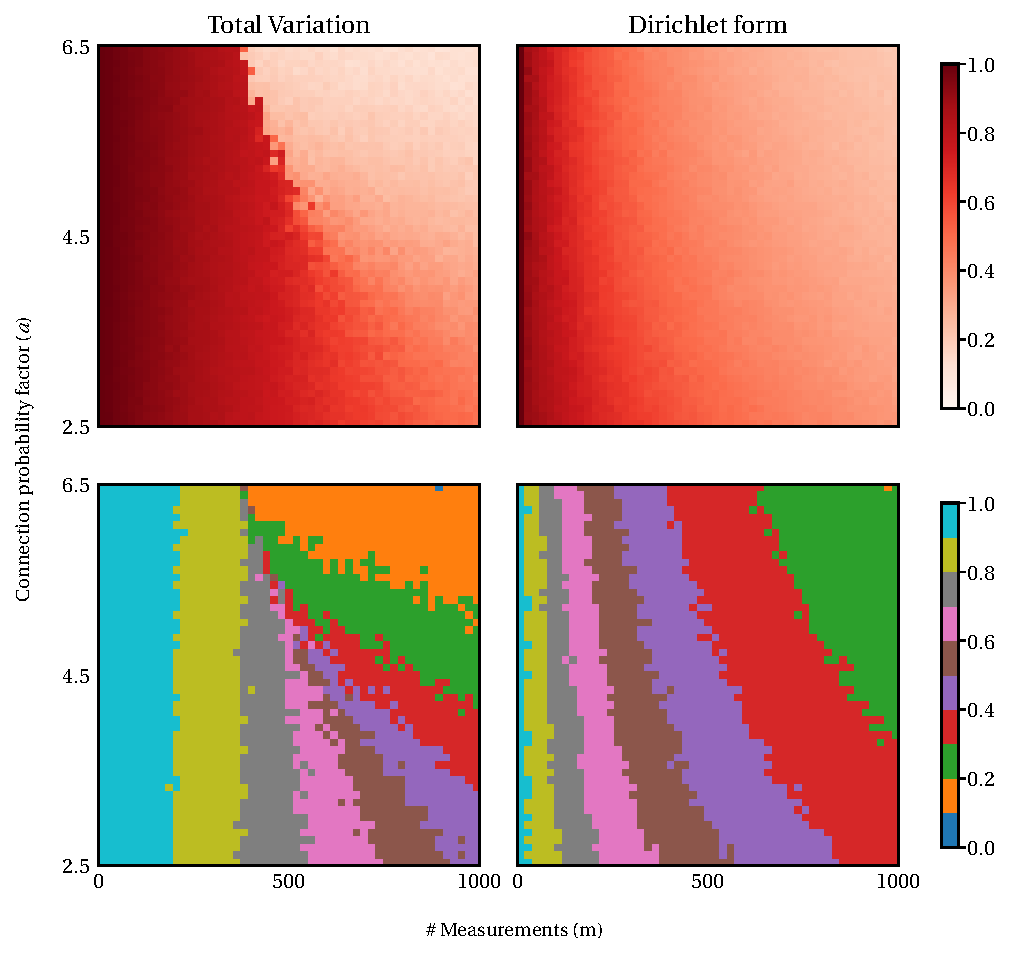
\includegraphics[width=0.95\textwidth]{pt_2sbm_unif_samp_tv_vs_dirichlet.pdf}
    \caption[Decoder's objective and the interpolation error: \texttt{2-SBM}(200~+~800)]{Effect of the decoder's objective on the interpolation error when recovering the indicator vector of the smallest community on \texttt{2-SBM}(200~+~800) graphs from samples taken uniformly at random. Left column: $\|\mathbf{Dz}\|_1$ (\acrlong{gtv} semi-norm). Right column: $\|\mathbf{Dz}\|_2^2$ (Dirichlet form). Each pixel on the top row represents the median, across 25 independent trials, of the normalized Euclidean distance from the recovered vector to the ground-truth. The bottom row has quantized versions of the plots from the top row, to better discern the error level-sets.}
    \label{fig:pt_2sbm_unif_samp_tv_vs_dirichlet}
\end{figure}

If we do the same comparison now using the \texttt{swiss-national-council} data, some of the same behaviors arise, but with interesting twists. See Figure \ref{fig:pt_snc_unif_samp_tv_vs_dirichlet}. The \acrshort{gtv} recovery error transitions sharply, but now this happens in two stages. My hypothesis for this behavior is that it is an artifact of the way I assembled the ground-truth signal. Although the UDC and FDP parties have a joint voting pattern that distinguishes them from the rest of the Council, these parties themselves do not vote identically in every affair. I suppose that the first drop in the error comes when the decoder approximately accounts for the largest, UDC component of the ground truth; the second drop would come when enough members of FDP are sampled as belonging to the same signal piece as UDC. The error in Dirichlet form interpolation does not change in stages; it decreases smoothly and is even smaller then the \acrshort{gtv} error in the beginning, just as in the previous experiment. The surprising observation this time is the error curves of the two decoders catching up at some point and proceeding to decrease smoothly at the same rate. The recovery errors to the right of the plot are still considerably large, but this might just be an indication that there are many councillors in the blue part of the ground-truth that vote very similarly to the UDC or FDP members. In other words, the large interpolation error is possibly a consequence of a large jump-set for the ground-truth signal.

\begin{figure}[H]
    \centering
    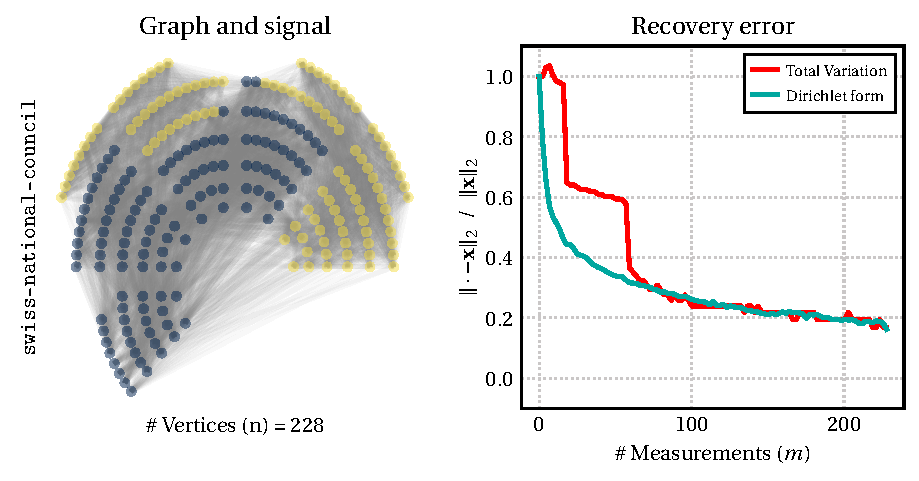
\includegraphics[width=\textwidth]{pt_snc_unif_samp_tv_vs_dirichlet.pdf}
    \caption[Decoder's objective and the interpolation error: \texttt{swiss-national-council}]{Effect of the decoder's objective on the interpolation error when recovering the indicator vector of the two largest right-wing parties (UDC and FDP) in the \texttt{swiss-national-council} graph from samples taken uniformly at random. \textcolor{epfl-groseille}{Red} curve: $\|\mathbf{Dz}\|_1$ (\acrlong{gtv} semi-norm). \textcolor{epfl-canard}{Blue} curve: $\|\mathbf{Dz}\|_2^2$ (Dirichlet form). Each point on the curves represents the median, across 51 independent trials, of the normalized Euclidean distance from the recovered vector to the ground-truth.}
    \label{fig:pt_snc_unif_samp_tv_vs_dirichlet}
\end{figure}


\section{Effects of the sampling design for \texorpdfstring{\acrshort{gtv}}{G-TV} interpolation}

At the end of Chapter \ref{ch:inexact_dual}, I gave an explicit expression for an optimal vertex-sampling design when working with the \acrshort{gtv} interpolation problem \eqref{eq:l1_interpolation}. It prescribes sampling probabilities $\bm{\pi}$ that minimize $\Gamma(\mathcal{S}, \bm{\pi})$, a functional that also depends on the jump-set $\mathcal{S} := \operatorname{supp}\left ( \mathbf{Dx} \right )$ of the signal-to-be-recovered. This optimization program is easy to state, but hard to implement, all due to the indirect definition of the objective as $\Gamma (\mathcal{S}, \bm{\pi}) := \max \{ \Theta (\mathcal{S}, \bm{\pi}), \Upsilon (\mathcal{S}, \bm{\pi})\}$. Out of the two random matrix moment estimates in the definition of $\Gamma$, it is $\Theta$ the one with the simplest expression. I will thus ignore $\Upsilon$ in this section and investigate sampling designs that minimize different upper bounds to $\Theta$, comparing their behavior with the baseline uniform random sampling.

To define the designs we will enquire into, recall Definition~\ref{def:sample_complexity_parameters} and consider the following succession of upper bounds for $\Theta(\mathcal{S}, \bm{\pi})$:
\begin{align}
    \Theta (\mathcal{S}, \bm{\pi}) & = \underset{i \in [n]}{\max} \enspace \underset{k \in [N]}{\max} \enspace \left \| \tilde{\mathbf{e}}_k^{\top} \left [ \mathbf{D} \left ( \mathbf{I}_n - \frac{1}{\pi_{i}}\mathbf{e}_{i} \mathbf{e}_{i}^\top \right ) \mathbf{D}^{+} \right ]^\top \mathbf{P}_{\mathcal{S}}\right \|_{1} \nonumber \\
    & \leq \underset{k \in [N]}{\max} \enspace \left \| \tilde{\mathbf{e}}_k^{\top} \left [ \mathbf{D} \mathbf{D}^{+} \right ]^\top \mathbf{P}_{\mathcal{S}}\right \|_{1} + \underset{i \in [n]}{\max} \enspace \underset{k \in [N]}{\max} \enspace \frac{1}{\pi_i} \left \| \tilde{\mathbf{e}}_k^{\top} \left [ \mathbf{D} \mathbf{e}_{i} \mathbf{e}_{i}^\top \mathbf{D}^{+} \right ]^\top \mathbf{P}_{\mathcal{S}}\right \|_{1} \nonumber \\
    & \leq \sqrt{N} + \underset{i \in [n]}{\max} \enspace \underset{k \in [N]}{\max} \enspace \frac{1}{\pi_i} \left | \tilde{\mathbf{e}}_k^{\top} (\mathbf{D}^{+})^{\top} \mathbf{e}_{i} \right | \cdot \left \| \mathbf{e}_{i}^\top \mathbf{D}^{\top} \mathbf{P}_{\mathcal{S}}\right \|_{1} \nonumber \\
    & = \sqrt{N}  + \underset{i \in [n]}{\max} \enspace \underset{k \in [N]}{\max} \enspace \frac{\left \| (\mathbf{D}^{+})^{\top} \mathbf{e}_{i} \right \|_{\infty} \cdot \left \| \mathbf{P}_{\mathcal{S}} \mathbf{D} \mathbf{e}_{i} \right \|_{1}}{\pi_i} \label{eq:jumpset_coherence_objective}  \\
    & \leq \sqrt{N} + \underbrace{\|\mathbf{P}_{\mathcal{S}} \|_{1 \to 1}}_{= |\mathcal{S}|} \cdot \underset{i \in [n]}{\max} \enspace \underset{k \in [N]}{\max} \enspace \frac{\left \| (\mathbf{D}^{+})^{\top} \mathbf{e}_{i} \right \|_{\infty} \cdot \left \| \mathbf{D} \mathbf{e}_{i} \right \|_{1}}{\pi_i}. \label{eq:naive_coherence_objective}
\end{align}
The sampling design $\bm{\pi}$ minimizing the bound in \eqref{eq:jumpset_coherence_objective} is the one that satisfies
\begin{equation}
    \pi_i = \frac{\left \| (\mathbf{D}^{+})^{\top} \mathbf{e}_{i} \right \|_{\infty} \cdot \left \| \mathbf{P}_{\mathcal{S}} \mathbf{D} \mathbf{e}_{i} \right \|_{1}}{\sum_{j=1}^{n} \left \| (\mathbf{D}^{+})^{\top} \mathbf{e}_{j} \right \|_{\infty} \cdot \left \| \mathbf{P}_{\mathcal{S}} \mathbf{D} \mathbf{e}_{j} \right \|_{1}}, \forall i \in [n].
    \label{eq:jump_set_coherence_probabilities}
\end{equation}
I call it the ``\emph{jump-set coherence}'' design, because it depends on the jump-set $\mathcal{S}$ --- through $\mathbf{P}_{\mathcal{S}}$ --- and on the coherence~\footnote{I use ``coherence'' here in the sense of \acrlong{cs}.} between $\mathbf{D}$ and the standard basis vectors in $\mathbb{R}^{n}$.~\footnote{Recall that our sampling matrix is a stack of standard basis vectors, so the quantified coherence is really between the analysis and measurement operators.} Note that this design is not necessarily practical, since it requires --- \emph{a priori} --- knowing the jump-set of the ``ground-truth'' graph signal. Another sampling design arises when we minimize the the looser bound in \eqref{eq:naive_coherence_objective}:
\begin{equation}
    \pi_i = \frac{\left \| (\mathbf{D}^{+})^{\top} \mathbf{e}_{i} \right \|_{\infty} \cdot \left \| \mathbf{D} \mathbf{e}_{i} \right \|_{1}}{\sum_{j=1}^{n} \left \| (\mathbf{D}^{+})^{\top} \mathbf{e}_{j} \right \|_{\infty} \cdot \left \| \mathbf{D} \mathbf{e}_{j} \right \|_{1}}, \forall i \in [n].
    \label{eq:naive_coherence_probabilities}
\end{equation}
It no longer depends on the jump-set of $\mathbf{x}$, but still has the coherence terms. I name this design ``\emph{naive coherence}'', because it is a consequence of naively controlling the jump-set $\mathcal{S}$ via its cardinality. Getting rid of the jump-set, though, has practical benefits: as long as we know the graph (represented in $\mathbf{D}$) we can implement the \emph{naive coherence} design. There is no need to consider the inaccessible ground-truth signal. But there are other designs that are simple to implement; uniform random sampling being arguably the simplest. \emph{Naive coherence} sampling only makes sense for our purposes if it implies a successful \acrshort{gtv} interpolation using fewer measurements than under uniform random sampling, and not many more than under the \emph{jump-set coherence} design. I contrast these three sampling strategies --- summarized on Table \ref{tab:summary_sampling_designs} --- in the set of experiments that follows.

\begin{table}[H]
    \centering
    \begin{tabularx}{0.6\textwidth}{rl}
        \hline
        Sampling design & Expression ($\forall i \in [n]$) \\
        \hline
        Uniform & $\pi_i = 1/n$ \\
        Naive coherence & $\pi_i \propto \left \| (\mathbf{D}^{+})^\top \mathbf{e}_i \right \|_{\infty} \cdot \left \| \mathbf{D} \mathbf{e}_i \right \|_1$ \\
        Jump-set coherence & $\pi_i \propto \left \| (\mathbf{D}^{+})^\top \mathbf{e}_i \right \|_{\infty} \cdot \left \| \mathbf{P}_\mathcal{S} \mathbf{D} \mathbf{e}_i \right \|_1$ \\
        \hline
    \end{tabularx}
    \caption[Summary of the three sampling designs compared in the experiments]{Summary of the sampling designs compared in the experiments. The expressions refer to the sampling probabilities $\bm{\pi} = (\pi_1, \dots, \pi_n)$ used in the \acrshort{cswr} model for vertex-sampling of graph signals (see Section~\ref{sec:sampling}).}
    \label{tab:summary_sampling_designs}
\end{table}

Let us begin by revisiting the \acrshort{sbm} datasets. Figure \ref{fig:pt_2sbm_tv_interp} shows the recovery error of \acrshort{gtv} interpolation under the three sampling designs, contrasting balanced and unbalanced community settings. We have already seen the plots from first column, but note how similar they are with the ones from the second column. The sample complexity for a correct output in \eqref{eq:l1_interpolation} under \emph{naive coherence sampling} is the same as if the vertices were sampled uniformly at random. The naive control over the ground-truth's jump-set is not enough to change the phase transition profile, a conclusion made all the more convincing once we examine the figure's third column. The change is subtle for the balanced \texttt{2-SSBM}(500~+~500) dataset, but very pronounced for the unbalanced case. Recovering the indicator vector unbalanced \texttt{2-SBM}(200~+~800) graphs is the naturally hard setting for the uniform sampling strategy, since the sampled vertices have only a one-in-four chance of belonging to the smallest community; in the balanced graphs, every other sample belongs to either community. The \emph{jump-set coherence} design seems to regularize the unbalanced signals, making the phase transition of their recovery look like the one for the symmetric \acrshort{sbm} under \emph{uniform random sampling}. The underlying cause of this regularization is found upon examining expression \eqref{eq:jump_set_coherence_probabilities}: only the vertices connected to edges on the ground-truth's jump-set are sampled with probability larger than zero.

\clearpage
\begin{figure}
    \centering
    \subfloat[\texttt{2-SSBM}(500~+~500)]{
        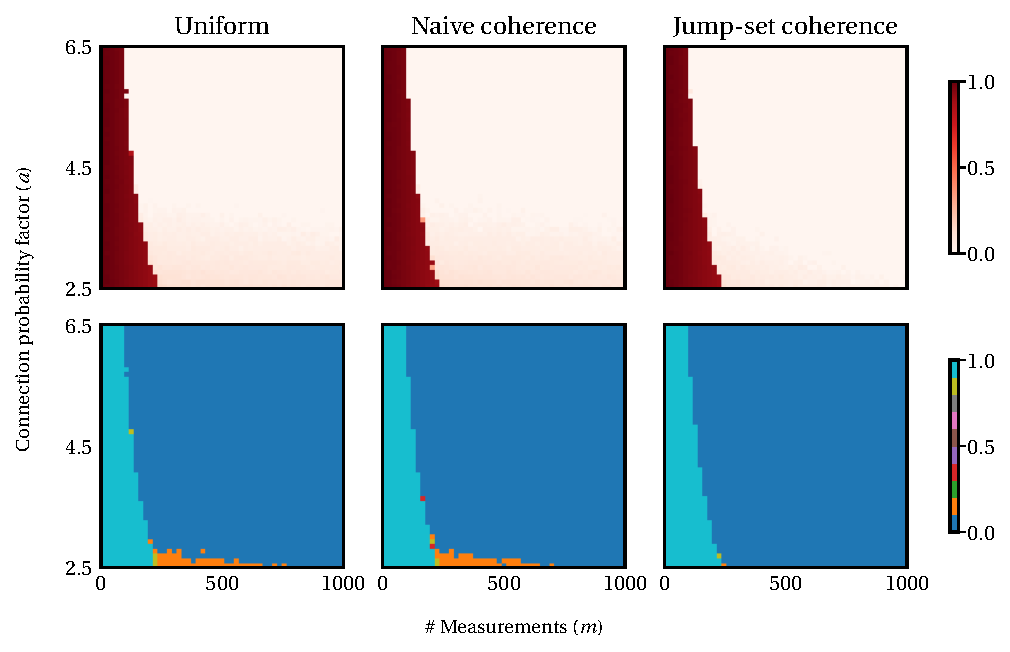
\includegraphics[width=0.95\textwidth]{pt_2ssbm_tv_interp.pdf}
    }
    \hfill
    \subfloat[\texttt{2-SBM}(200~+~800)]{
        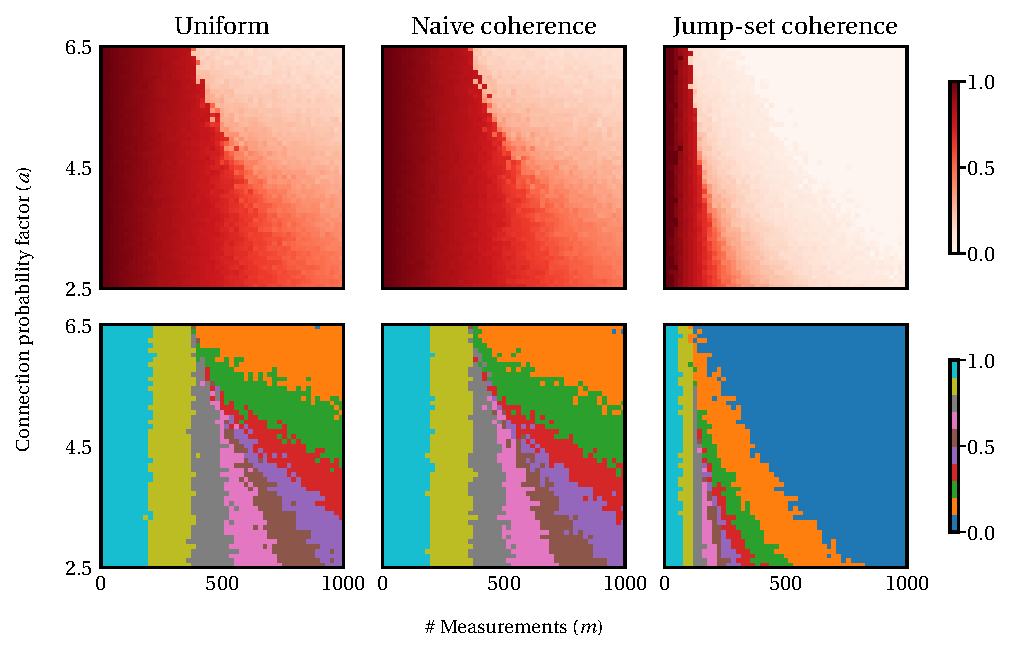
\includegraphics[width=0.95\textwidth]{pt_2sbm_tv_interp.pdf}
    }
    \caption[Three sampling designs: \texttt{2-SSBM}(500~+~500) and \texttt{2-SBM}(200~+~800)]{Impact of three sampling designs on the recovery error of \acrshort{gtv} interpolation for the community indicator vectors of \acrshort{sbm} graphs. Each pixel represents the median error over 25 independent trials. Each plot is paired with its quantized version highlighting some error level-sets.}
    \label{fig:pt_2sbm_tv_interp}
\end{figure}
\clearpage

We can draw similar conclusions for the effects of the three sampling designs using the ``real-world'' datasets \texttt{email-EU-core} and \texttt{swiss-national-council}, but we find also some surprises. Figure~\ref{fig:pt_email_snc_tv_interp} shows that once again the \emph{naive coherence} design behaves just as poorly as \emph{uniform random sampling}; the red curves are more intriguing.

\begin{figure}[H]
    \centering
    \subfloat[Ground-truth: indicator vector of the 5 largest departments]{
        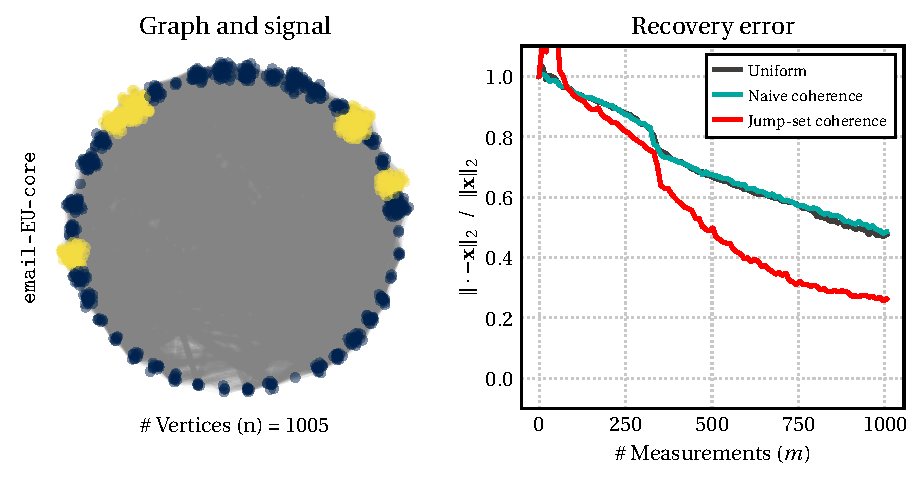
\includegraphics[width=0.95\textwidth]{pt_email_eu_core_tv_interp.pdf}
    }
    \hfill
    \subfloat[Ground-truth: indicator vector of the 2 largest right-wing parties]{
        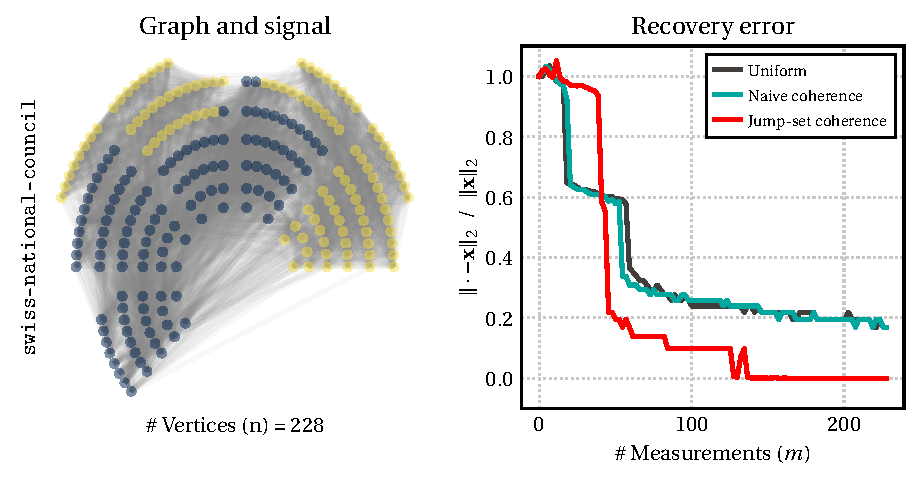
\includegraphics[width=.9\textwidth]{pt_snc_tv_interp.pdf}
    }
    \caption[Three sampling designs: \texttt{email-EU-core} and \texttt{swiss-national-council}]{Impact of three sampling designs on the recovery error of \acrshort{gtv} interpolation for the signals of the \texttt{email-EU-core} and \texttt{swiss-national-council} datasets. Each point in the plot represents the median error over 51 independent trials.}
    \label{fig:pt_email_snc_tv_interp}
\end{figure}
\clearpage

On the plots of Figure~\ref{fig:pt_email_snc_tv_interp}, the \emph{jump-set coherence design} reaches smaller recovery errors than the ones of the two others, but when the measurements are very few this design's error becomes the largest. I think this has do with with how well the ground-truth's jump-set reflects the natural partitions of the graph. When the \acrshort{gtv} decoder has very few measurements, it must rely almost only on the graph structure to do the interpolation. For the \acrshort{sbm} datasets this dependence was not detrimental because the signals being recovered were really the indicator vectors of the natural communities in the graphs. For the \texttt{email-EU-core} and \texttt{swiss-national-council} datasets I constructed assembled the ground-truth based only on an intuitive idea of how the respective graphs would cluster. When sampling a few vertices, only at the signal transitions, the \emph{jump-set coherence design} may lack the sample variety of the other designs that suggests the \acrshort{gtv} decoder should settle for a less-than-natural partition of the graph. In the end, however, the role of the graph in recovery problems like ours is to \emph{inform} the composition of the signal; very rarely in practice does the graph encode \emph{exactly} a signal of interest. The fact that the \emph{jump-set coherence design} reaches --- globally --- lower error levels than the other two designs is more important. After all, the error values to the left of the plot are \emph{all} very large. To the right --- as the number of samples increases---, the \emph{jump-set coherence design} even results in exact recovery for the \texttt{swiss-national-council} data, hinting that the voting patterns of the Swiss National Councillors reflect their political leaning better than the email exchanges in the \texttt{email-EU-core} reflect the institution's departmental makeup.

To finish off, let us sweep the \texttt{BSDS300} dataset and compare the error curves for the three sampling designs when recovering the segmentation mask graph signals. Figure \ref{fig:pt_bsds300_tv_interp} displays these side-by-side, with a gray curve for each image in the dataset.

\begin{figure}[H]
    \centering
    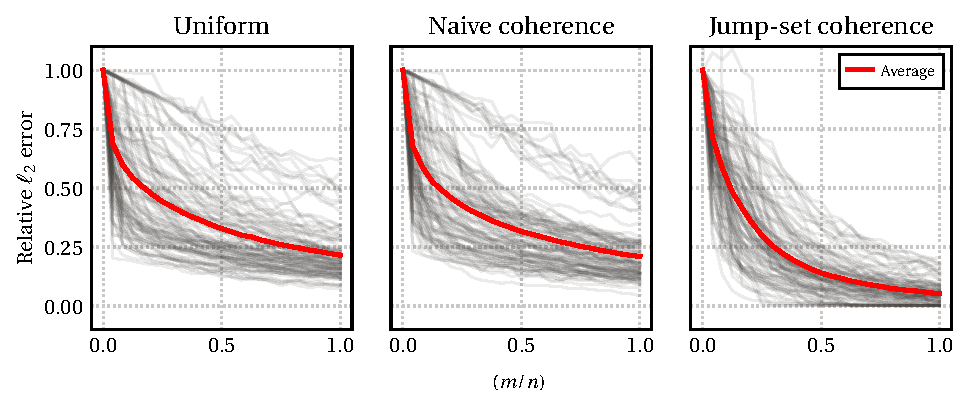
\includegraphics[width=\textwidth]{pt_bsds300_tv_interp.pdf}
    \caption[Three sampling designs: \texttt{BSDS300}]{Impact of three sampling designs on the recovery error of \acrshort{gtv} interpolation for the segmentation masks in \texttt{BSDS300}. Each grey curve on each of the three plots corresponds to an image in the dataset. Each point in these curve records the median error over 15 independent trials. The red curve traces the point-wise average the grey ones.}
    \label{fig:pt_bsds300_tv_interp}
\end{figure}

Note first that not every image in the dataset admits a sharp phase transition in the recovery error. For some, the error drops suddenly at a critical number of samples; for others the error decreases smoothly and remains large even when a lot of pixels are queried. For the first time in our experiments one could argue that there is \emph{some} improvement in using the \emph{naive coherence design} over uniform random sampling, but not enough to justify its use. The \emph{jump-set coherence design} leads to exact recovery for some segmentation masks, but for others the recovery error remains fairly large despite the use of unfair knowledge about the ground-truth jump-set in the sampling design. Let us examine the images associated with extremes of this behavior to see where this disparity comes from. The left column of Figure~\ref{fig:bsds300_imgs_smallest_largest_error} shows the image whose segmentation mask leads to the smallest recovery error under \emph{jump-set coherence sampling}; the right column shows the image with the largest respective error. The larger error seems to have to do with with the presence of several small pieces in the image's segmentation. Even when the sampling design is restricted to query only vertices belonging to the jump-set, it can still miss samples from some of the several small segments.

\begin{figure}[H]
    \centering
    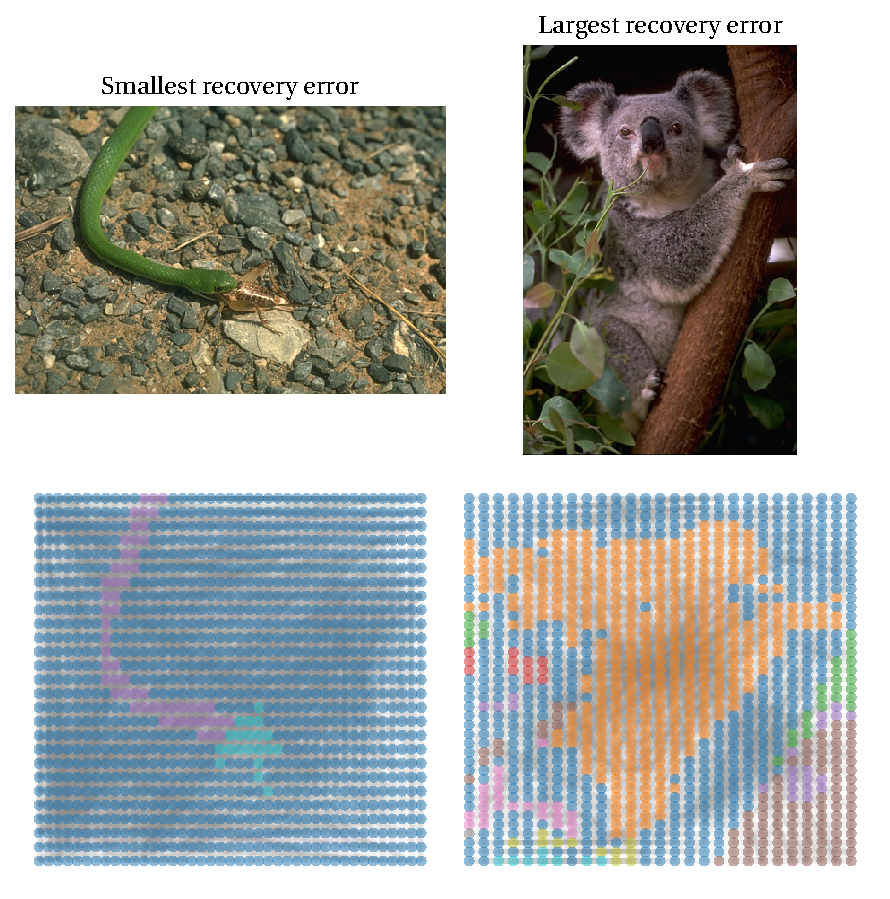
\includegraphics[width=0.7\textwidth]{bsds300_imgs_smallest_largest_error.pdf}
    \caption[Segmentation masks in \texttt{BSDS300} with the smallest and largest recovery errors]{Segmentation mask signals in the \texttt{BSDS300} dataset that yield the smallest and largest recovery errors when taking $m = n$ samples (with replacement) under the \emph{jump-set coherence design}.}
    \label{fig:bsds300_imgs_smallest_largest_error}
\end{figure}
\clearpage


\section{Summary}

The thorough study of a recovery program should not ignore the issues involved in its practical use. Fortunately, the \acrshort{gtv} decoders in \eqref{eq:l1_interpolation} and \eqref{eq:l1_regression} can be implemented numerically in efficient ways. The one I presented is based on a single primal-dual proximal splitting procedure whose iterations required, in the end, operations that can be made cheaper the sparser the graph is. Upon convergence, the estimated solution can be close or far to the true underlying signal, depending on the number of vertex-samples taken. I have shown that when the ground-truth is the indicator vector of a graph cluster, the recovery error of \acrshort{gtv} interpolation undergoes a sharp phase transition with respect to the number of samples. The threshold happens earlier the denser are the clusters. In contrast, the error under Dirichlet form interpolation when recovering these signals decreases smoothly and slowly, depending more on the actual number of measurements than on the edge structure of the graph.

Putting into practice the optimal sampling design for \acrshort{gtv} interpolation also has issues of its own. In an effort to simplify the complicated objective of the optimal design, I proposed for it two progressively looser upper bounds, whose optimizers gave rise to two sampling designs. Both are a form of coherence sampling, familiar in \acrlong{cs}, but one of them also uses information from the jump-set of the ground-truth signal. I compared these two designs with the baseline uniform random sampling, concluding that some information about the ground-truth's jump-set must be used in order to change the phase transition profile of the recovery error in \acrshort{gtv} interpolation; \emph{naive coherence sampling} behaves just as poorly as \emph{uniform random sampling}. The practical issue that remains is how to account for the jump-set in the sampling designs without actually resorting to the --- \emph{unknowable} --- ground-truth signal?

\clearpage

\begin{subappendices}
    \section{More on primal-dual proximal splitting}\label{ap:primal_dual_prox_split}
    In this appendix I sketch, in a little more detail than in the main text, the proximal splitting approach for numerically solving programs like the \acrshort{gtv} decoders \eqref{eq:l1_interpolation} and \eqref{eq:l1_regression}. We may consider here more general optimization problems of the type
\begin{equation}
    \underset{\mathbf{z} \in \mathbb{R}^{n}}{\min} \enspace f(\mathbf{z}) + g(\mathbf{Dz}) + h(\mathbf{z}),
    \label{eq:opt_prob_std_form} \tag{$P_{\text{std}}$}
\end{equation}
where $f: \mathbb{R}^{n} \to \mathbb{R}$, $g: \mathbb{R}^{N} \to \mathbb{R}$ and $h: \mathbb{R}^{n} \to \mathbb{R}$ are convex functions, the latter of which is also differentiable (with a Lipschitz-continuous gradient).

The proximity operator of a convex function $f : \mathbb{R}^{n} \to \mathbb{R}$ is the map
\begin{equation}
    \mathbf{z} \mapsto \operatorname{prox}_{f} \left ( \mathbf{z} \right ) = \text{arg} \enspace \underset{\mathbf{v} \in \mathbb{R}^{n}}{\min} \enspace \frac{1}{2} \|\mathbf{z} - \mathbf{v} \|_2^2 + f(\mathbf{v}).
\end{equation}
The problem on the \acrlong{rhs} admits a unique solution for every $\mathbf{z} \in \mathbb{R}^{n}$. One can interpret proximity operators as generalizing projections. Indeed, take $f$ to be the convex indicator function of a set $\mathcal{C}$, \ie, the functions defined by
\begin{equation*}
    \mathbf{z} \mapsto \iota_{\mathcal{C}}(\mathbf{z}) = \left \{
        \begin{matrix}
            0, & \text{if }\mathbf{z} \in \mathcal{C}, \\
            +\infty & \text{otherwise}
        \end{matrix}
    \right. .
\end{equation*}
Then, for any $\mathbf{z} \in \mathbb{R}^{n}$, the vector $\operatorname{prox}_{f} \left ( \mathbf{z} \right )$ is exactly the orthogonal projection of $\mathbf{z}$ onto $\mathcal{C}$~\cite[Table~2,~entry~i]{combettes2011}. Just like orthogonal projections, proximity maps allow us to split the space into complementary halves. Given a convex function $f$, the so-called Moreau decomposition of any $\mathbf{v} \in \mathbb{R}^{n}$ is given by
\begin{equation*}
    \mathbf{v} = \operatorname{prox}_{f} \left ( \mathbf{v} \right ) + \operatorname{prox}_{f^*} \left ( \mathbf{v} \right ),
\end{equation*}
where $f^*$ is the Fenchel conjugate of $f$, a function defined as $\mathbf{v} \mapsto \underset{\mathbf{u} \in \mathbb{R}^{n}}{\sup} \enspace \langle \mathbf{u}, \mathbf{v} \rangle - f(\mathbf{u})$.

But perhaps the two most important properties of $\operatorname{prox}_{f}$ --- in what concerns iterative solvers --- are its firm non-expansiveness and the fact that its fixed point set matches the set of minimizers of $f$~\cite{combettes2011}. The gradient descent map $\mathbf{w} \mapsto \mathbf{w} - \gamma \nabla h (\mathbf{w})$ can also be non-expansive (with a proper choice of step size $\gamma$) and, similarly to the proximity map, its fixed point set is equal to the set of minimizers of $h$. \emph{Proximal splitting} techniques take advantage of these two properties to solve problems of the type $\underset{\mathbf{z}}{\min} \enspace f(\mathbf{z}) + h(\mathbf{z})$ with alternating calls to the gradient of $h$ (forward step) and proximal operator of $f$ (backward step). In rough terms, the iterations look like the ones below and repeat until $\mathbf{z}$ stops changing noticeably, coming close enough to a minimizer of the sum $f(\cdot) + h(\cdot)$.
\begin{algorithm}[H]
    \begin{algorithmic}
        \State{$\mathbf{z} \gets \mathbf{z} - \gamma \nabla h (\mathbf{z})$}\Comment{Forward step}
        \State{$\ldots$}
        \State{$\mathbf{z} \gets \operatorname{prox}_{\gamma f} \left ( \mathbf{z} \right )$}\Comment{Backward step}
    \end{algorithmic}
\end{algorithm}

Adding $g$ to the objective changes things a bit, because the domain of this function is different from that of $f$ and $h$. \emph{Primal-dual} proximal splitting methods address this situation by working simultaneously with two variables, called the primal $\mathbf{z} \in \mathbb{R}^{n}$ and the dual $\mathbf{d} \in \mathbb{R}^{n}$. The direct linear map $\mathbf{z} \mapsto \mathbf{D}\mathbf{z}$ and its transpose, $\mathbf{d} \mapsto \mathbf{D}^\top \mathbf{d}$ connect the primal and dual domains between the forward and backward steps:
\begin{algorithm}[H]
    \begin{algorithmic}
        \State{$(\mathbf{z}, \mathbf{d}) \gets \left(\mathbf{z} - \gamma \nabla h (\mathbf{z}) - \gamma \mathbf{D}^\top \mathbf{d}, \mathbf{d} + \gamma \mathbf{D} \mathbf{z}\right)$}\Comment{Forward step}
        \State{$\ldots$}
        \State{$(\mathbf{z}, \mathbf{d}) \gets \left(\operatorname{prox}_{\gamma f} \left ( \mathbf{z} \right ), \operatorname{prox}_{\gamma g^*} \left ( \mathbf{d} \right )\right)$}\Comment{Backward step}
    \end{algorithmic}
\end{algorithm}

The specific primal-dual proximal splitting method used in this chapter comes from Komodakis~and~Pesquet~\cite[Algorithm~6]{komodakis2015}. I reproduce all of its steps in Algorithm \ref{algo:primal_dual_general}, but note that at its core the algorithm consists of forward gradient steps, backward proximity steps, and a linear connection between primal and dual spaces via matrix $\mathbf{D}$. The paper of Komodakis~and~Pesquet lists other numerical solvers for \eqref{eq:opt_prob_std_form}, but the one in Algorithm~\ref{algo:primal_dual_general} has more intuitive step size parameters and allows the computation of $\operatorname{prox}_{f}$ and $\operatorname{prox}_{g}$ in parallel.

\begin{algorithm}
    \caption{\acrshort{fbf} primal-dual iterations for solving \eqref{eq:opt_prob_std_form}}
    \label{algo:primal_dual_general}
    \begin{algorithmic}[1]
        \State{$\mathbf{z}_0 \gets \mathbf{0} \in \mathbb{R}^{n}$}\Comment{Initial primal variable}
        \State{$\mathbf{d}_0 \gets \mathbf{0} \in \mathbb{R}^{N}$}\Comment{Initial dual variable}
        \Repeat
            \State{\textbf{pick} $\gamma_n \in \left(0, \frac{1}{1 + \|\mathbf{D}\|_{2} + \rho}\right)$}\Comment{Step size}

            \State{$\left(\mathbf{w}_{1,n},\enspace\mathbf{w}_{2,n}\right) \gets \left(\mathbf{z}_n - \gamma_n \left[\nabla h (\mathbf{z}_n) + \mathbf{D}^\top \mathbf{d}_n\right],\enspace\mathbf{d}_n + \gamma_n \mathbf{D}\mathbf{z}_n\right)$}\Comment{Forward step}

            \State{$\left(\mathbf{p}_{{1,n}},\enspace\mathbf{p}_{{2,n}}\right) \gets \left(\operatorname{prox}_{\gamma_n f} \left ( \mathbf{w}_{1,n} \right ),\enspace\operatorname{prox}_{\gamma_n g^*} \left ( \mathbf{w}_{2,n} \right )\right)$}\Comment{Backward step}

            \State{$\left(\mathbf{q}_{{1,n}},\enspace\mathbf{q}_{{2,n}}\right) \gets \left(\mathbf{p}_{{1,n}} - \gamma_n \left[ \nabla h (\mathbf{p}_{{2,n}}) + \mathbf{D}^\top \mathbf{p}_{{2,n}}\right],\enspace\mathbf{p}_{{2,n}} + \gamma_n \mathbf{D} \mathbf{p}_{{1,n}}\right)$}\Comment{Forward} step

            \State{$\left(\mathbf{z}_{n+1},\enspace\mathbf{d}_{n+1}\right) \gets \left(\mathbf{z}_n - \mathbf{w}_{1,n} + \mathbf{q}_{1,n},\enspace\mathbf{d}_n - \mathbf{w}_{2,n} + \mathbf{q}_{2,n}\right)$}\Comment{Update primal/dual variables}

        \Until{convergence}
        \State{\textbf{return} $\mathbf{z}_{n+1}$}
	\end{algorithmic}
\end{algorithm}

Algorithms \ref{algo:primal_dual_interpolation} and \ref{algo:primal_dual_regression} in the main text are straightforward specializations of Algorithm \ref{algo:primal_dual_general}. To see that this is true, first identify $g$ with $\|\cdot\|_1 : \mathbb{R}^{N} \to \mathbb{R}$. Then the proximal mapping of its Fenchel conjugate is given by
\begin{align*}
    \mathbf{w} \mapsto & \operatorname{prox}_{\gamma_n g^*} \left ( \mathbf{w} \right ) \\
    & = \mathbf{w} - \operatorname{prox}_{\gamma_n g} \left ( \mathbf{w} \right ) \\
    & = \mathbf{w} - \operatorname{soft}_{\gamma_n} (\mathbf{w}).
\end{align*}
Note that I used the Moreau decomposition, along with the fact that $\operatorname{prox}_{\gamma_n \|\cdot\|_1}$ is the soft thresholding operator $\operatorname{soft}_{\gamma_n} (\mathbf{w})$~\cite[Table 2, entry ii]{combettes2011}. Next, in the interpolation problem related to Algorithm~\ref{algo:primal_dual_interpolation}, we have $h \equiv 0$ and so $\nabla h \equiv \mathbf{0}$. The interpolation constraint is expressed via function $f$ with the convex indicator function $\iota_{\{\mathbf{z} \in \mathbb{R}^{n} : \mathbf{P}_{\Omega}\mathbf{z} = \mathbf{P}_{\Omega}\mathbf{x}\}}(\cdot)$. Its proximity map is the same as the orthogonal projection onto set $\{\mathbf{z} \in \mathbb{R}^{n} : \mathbf{P}_{\Omega}\mathbf{z} = \mathbf{P}_{\Omega}\mathbf{x}\}$:
\begin{align*}
    \mathbf{w} \mapsto & \operatorname{prox}_{\gamma_n f} \left ( \mathbf{w} \right ) \\
    & = \text{arg} \enspace \underset{\{ \mathbf{z} \in \mathbb{R}^{n} : \mathbf{P}_{\Omega} \mathbf{z} = \mathbf{P}_{\Omega} \mathbf{x} \}}{\min} \enspace \|\mathbf{z} - \mathbf{w}\|_2 \\
    & = (\mathbf{I}_n - \mathbf{P}_{\Omega}) \mathbf{w} + \mathbf{P}_{\Omega}\mathbf{x}.
\end{align*}
For the regression problem, we can express the constraints using a differentiable function, $h(\cdot) = \frac{\rho}{2} \| \mathbf{P}_{\Omega}(\cdot) - \mathbf{y}\|_2^2$. Its corresponding gradient map is $\mathbf{z} \mapsto \nabla h (\mathbf{z}) = \rho \mathbf{P}_{\Omega}^\top \mathbf{P}_{\Omega}\mathbf{z} - \mathbf{y} = \rho \mathbf{P}_{\Omega}\mathbf{z} - \mathbf{y}$. There is no need for another function in the objective, so we may set $f \equiv 0$, which finishes the specialization of Algorithm \ref{algo:primal_dual_general} into Algorithm~\ref{algo:primal_dual_regression}.
\end{subappendices}